%\begin{savequote}[8cm]
%\textlatin{Jedem Anfang wohnt ein Zauber innne.}
%
%In the core of every beginning lives magic.
%  \qauthor{--- Hermann Hesse's \textit{Stufen}}
%\end{savequote}

\chapter{\label{ch:5-experiments}Experiments} 

%\minitoc

\section{Deep Counterfactual Networks}
In chapter \ref{ch:3-DCNs} we introduced \emph{deep counterfactual networks} (DCN) with a propensity-based dropout scheme (PD) for the task of counterfactual inference. In the following, we will run a number of experiments on the model to evaluate its performance and compare it to a variety of baseline methods and existing competing approaches. 

Firstly, we introduce the dataset that we are running the experiments on before describing the experimental setup in detail including the used hyper-parameters and relevant implementation details. Finally, we show the results of the experiments provide a discussion of the outcomes and its implications.  

\subsection{Dataset}
As described in section \ref{sec:counterfactual-inference}, due to the very nature of counterfactual inference we are never able to access the ground truth for the counterfactual outcomes for any observational dataset. This poses an enormous challenge when it comes to evaluating the performance of any model used for causal inference on real-world data. In order to deal with this issue, we follow (Hill) % CITE Hill, Johansson..
and adopt a \emph{semi-synthetic} experimental setup for which we use the actual covariates and treatment assignments from the dataset but simulate the outcomes in order to have access to both the factual and the counterfactual outcomes. Nonetheless, it is important to note that the counterfactual outcome is only used for evaluation purposes and considered as unavailable during training time. 

The experiments are conducted on the Infant Health and Development Program (IHDP) dataset that was introduced in (Hill, 2012). % CITE Hill
 program that was carried out in the second half of the 1980s tried to aid premature infants at an early age to enhance their cognitive abilities measured in terms of the IQ score. The dataset consists of a total of 747 subjects out of which 139 were treated and 608 controlled. Each subject has 6 continuous and 19 binary features representing attributes of the child such as birth weight, sex, and weeks born pre-term, and relevant attributes of the mother measured around the time of giving birth (e.g. age, educational status, etc.). The outcome are simulated based on a functions that are described as "Response Surface B" setting in (Hill, 2012). % CITE HILL 2012
 

\subsection{Experiment Setup} \label{sec:pbd-experiment-setup}
We are evaluating the performance of a \emph{deep counterfactual network} with \emph{propensity-dropout} which we will refer to as DCN-PD. In our experiment we are using an architecture with $L_s = 2, L_{i,0} =2 , L_{i,1} = 2$, thus $L_{\text{total}} = 4$ total layers, % IMPORTANT Do we consider the depth or the sum of layes as total? Shouldn't it be 6 instead?
and utilise a fixed number of $h_s^{(l)} = h_{i,0}^{(l)} = h_{i,1}^{(l)} = 200$ hidden units for the $l^{th}$ layer in the network. We are using a ReLU activation function for our network and we evaluate the performance of the model in terms of the mean squared error (MSE)
% EQUATION Make sure this is correct!
\begin{equation} \label{eq:mse-ite}
\text{MSE} = \frac{1}{n}\sum_{i=1}^{n} (T_i(x) - \tilde{T}_i(x))^2 = \frac{1}{n}\sum_{i=1}^{n} ((Y_i^{(1)} - Y_i^{(0)}) - (\tilde{Y}_i^{(1)} - \tilde{Y}_i^{(0)}))^2
\end{equation}
 of the estimated treatment effect and the true treatment effect (as defined in equation \ref{eq:ite}).  

The IHDP dataset is split into a training set comprising 80\% of the data and a test set with the remaining 20\%. We run a total of $N_E = 100$ experiments, each time drawing new outcomes according to the data generation model described in (Hill, 2012), % CITE Hill
and report the average MSE across all experiments, each time evaluated exclusively on the out-of-sample test set. 

For the \emph{propensity network} (see \ref{sec:multi-task-learning}) that is used to estimate the propensity scores for each subject, we used $L_p = 2$ layers with $h_p^{(l)}) = 25$ hidden units per layer, trained using an Adam optimiser % CITE ADAM 
and Xavier initialisation. % CITE XAVIER
The propensity-dropout is applied as described in section \ref{sec:propensity-based-dropout} and uses $\lambda = 1$. 

% TODO Should I mention Tensorflow? 
%The neural network is implemented in Tensorflow %CITE TEnsorflow
\subsection{Results and Discussion}
Firstly, we investigate the impact of our propensity-dropout scheme by comparing a DCN-PD to other deep counterfactual networks with regular dropout schemes (that is the dropout probability is fixed throughout all samples and for the hidden units in all layers). Figure \ref{fig:propensity-dropout-boxplot} shows the marginal gains in terms of the MSE achieved by the DCN-PD (right) over a DCN with a dropout probability $p=0.2$ (middle), and a DCN with dropout probability $p=0.5$ (left) in form of a box plot. 



%As we can see in Fig. 3, the DCN- PD model offers a significant improvement over the two DCN models for which the dropout probabilities are uni- form over all the training examples. This result implies that the DCN-PD model generalizes better to the true fea-
%Figure 3. Performance gain achieved by propensity-dropout.
%ture distribution when trained with a biased dataset as com- pared to DCN with regular dropout, which suggests that propensity-dropout is a good regularizer for causal infer- ence.


\begin{figure}[h]
	\centering
	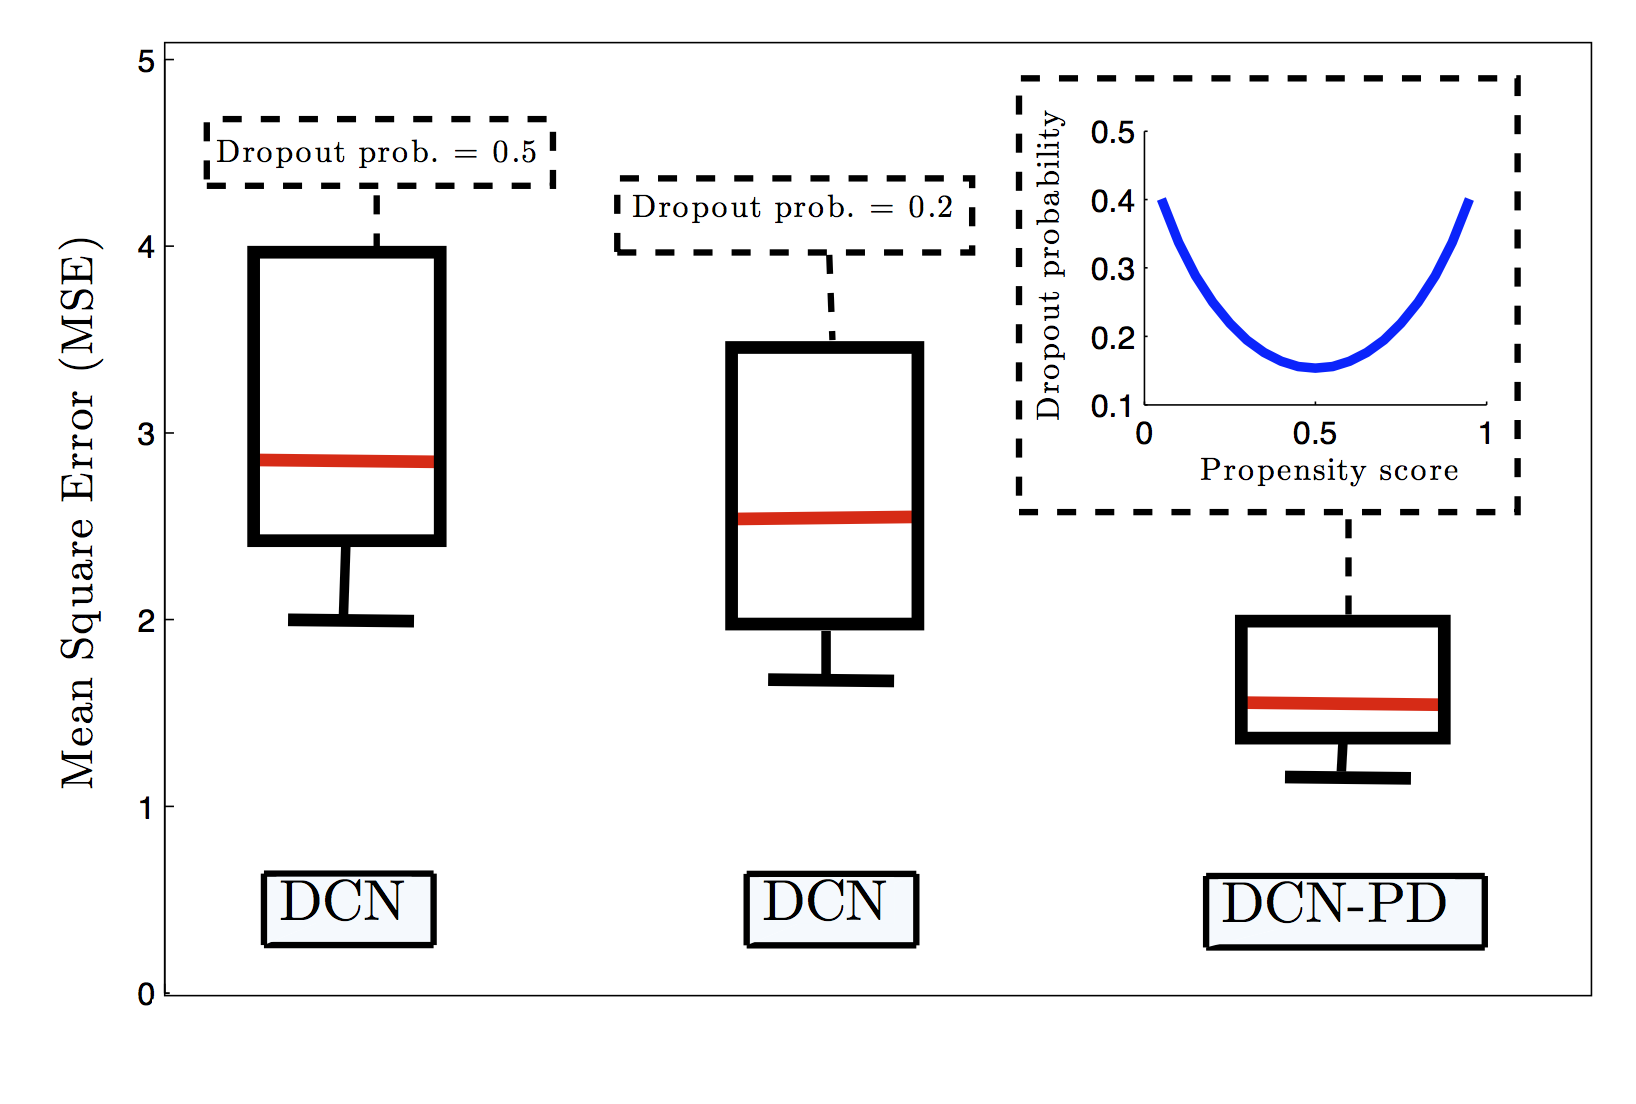
\includegraphics[width=0.9\textwidth]{figures/chapter-5/pd-boxplot.png}
	\caption{Comparison between the performance of a DCN with propensity-based dropout (right) and DCNs with regular dropout schemes (middle, left) in terms of the mean squared error (lower is better). The propensity-dropout has a regularising effect towards the selection bias and provides the model a higher degree of generalisation. }\label{fig:propensity-dropout-boxplot}
\end{figure}

As we can observe in the figure, our propensity-based dropout scheme provides a significant improvement over the alternative DCNs for which the  dropout probabilities are uniform throughout all samples in the training set. The result implies that the propensity-based dropout helps the DCN to generalise better to the true feature distribution when trained with an biased dataset such as IHDP (139 treated vs. 608 controlled subjects). Consequently, this suggest that propensity-dropout can be an effective regulariser for the task of counterfactual inference. 

In the following, we will look at the performance of a DCN and DCN-PD in comparison to competing state-of-the-art methods shown in table \ref{tab:dcn-pd-results}. Concretely, we compare the mean MSE (aggregated over $N_E = 100$ experiments) that is achieved by our models to the MSE of k-Nearest-Neighbour matching (k-NN), Causal Forests with double-sample tree (WagerAthey, 2015), % CITE Wager Athey
a classical feed-forward neural network with the treatment assignemnt as input feature (NN-4),
Bayesian Additive Regression Trees (BART) (Chipman) % CITE CHipman, Hill
and balancing neural networks (BNN) (Johanson) % CITE JOhannson
that we discussed in detail in section \ref{sec:representation-learning} and which represent the state-of-the-art for counterfactual inference. 
In order to ensure a fair comparison, for the BNN and the NN-4 we are also using $4$ layers, each with $200$ hidden units trying to hold as many hyper-parameters as possible constant. The DCN uses regular dropout scheme with a dropout probability of $p=0.2$ and the DCN-PD is regularised using our propensity-based dropout.

As we can see in table \ref{tab:dcn-pd-results}, the DCN-PD achieves the lowest MSE and outperforms the other methods. The BNN, representing  a strong benchmark as it effectively handles the selection bias by learning a balanced representation for the input features, represents the most competitive alternative. Lastly, the performance gains that our DCN-PD achieves over a the NN-4 model suggest that the multi-task learning framework is an effective conception of counterfactual inference that outperforms direct modelling approaches which consider the treatment assignment as a regular input feature.   %TODO Should I mention that DCNs don't perform too wel? 

Concluding, it can be said that our proposed model of deep counterfactual networks using propensity-dropout (DCN-PDs) represents a promising approach to using deep neural networks for counterfactual inference that it is able to compete with and potentially even outperform existing methods. 

% TODO Mention criticm ? 

\begin{table}[]
	\centering
	\begin{tabular}{@{}cc@{}}
		\toprule
		\textbf{Algorithm} & \textbf{MSE}                \\ \midrule
		k-NN               &   $5.30 \pm 0.30$           \\
		Causal Forest      &   $3.86 \pm 0.20$           \\
		BART               &   $3.50 \pm 0.20$           \\ 
		BNN                &   $2.45 \pm 0.10$           \\
		NN-4                &  $2.88 \pm 0.10$           \\
		DCN                &   $2.58 \pm 0.06$           \\
		DCN-PD             &   $2.05 \pm 0.03$          \\\bottomrule
	\end{tabular}
	\caption{Performance of Deep Counterfactual Networks (DCN) and Deep Counterfactual Networks with Propensity-Dropout (DCN-DP) in comparison with baseline methods and existing competing approaches}\label{tab:dcn-pd-results}
\end{table}


\section{Architecture Learning for DCN}
In chapter \ref{ch:4-DCN-LAs} we introduced an efficient approach to automatically infer an appropriate architecture for \emph{deep counterfactual networks} (DCN) without the need for computationally expensive hyper-parameter optimisation (e.g. grid search, random search, or bayesian optimisation). 

In the following, we will run a number of experiments to investigate the performance of the model with the inferred architecture. In particular, we investigate how the different characteristics (selection bias, shared complexity, and outcome-specific complexity) that we defined in section \ref{sec:relevant-characteristics} influence the learnt architecture and the performance of the model. 

Firstly, we introduce a purely synthetic dataset that gives us full control over the relevant characteristics, and a real-world dataset for which the characteristics have to be inferred according to our approach. Thereafter, we describe the experimental setup in detail including the used hyper-parameters and relevant implementation details before showing the results of the experiments and concluding with a discussion of the outcomes and its implications.  


\subsection{Datasets}
\subsubsection{Synthetic Model} \label{sec:synthetic-model}
For the synthetic model, we draw $n = 1000$ samples in the form of a tuple $\langle X_i, W_i, Y_i \rangle$ for each subject $i$. Each $X_i = (x_{i,0}, x_{i,1}, \ldots, x_{i,24})$ consists of $d = 25$ covariates for each subject which are independently drawn from a uniform distribution, i.e.  

\begin{equation}
x_{i,0}, x_{i,1}, \ldots, x_{i,24} \overset{iid}{\sim} \mathcal{U}(0, 1)
\end{equation}
keeping each covariate strictly non-negative. For the treatment assignment indicator $W_i \in \{0,1\}$, we define

\begin{equation}
\tilde{p}(X_i) =  \frac{1}{1 + exp(- \alpha\sum \limits_{{x_{j} \in X_i}} x_j)} % \mathbb{P}(W_i = 1 \mid X_i = x) =
\end{equation}
\begin{equation}
W_i \sim Bernoulli(\tilde{p}(X_i))
\end{equation}
where $\tilde{p}(X_i)$ represents the subject's propensity score and the parameter $\alpha \in \mathbb{R}_{\geq0}$ gives us a way to control the imbalance between the treated and untreated subjects. For $\alpha = 0$, we get $\tilde{p}(X_i) = 0.5$ corresponding to a maximum balance between the number of treated and untreated subjects whereas an increasing alpha shifts the distribution towards a higher proportion of treated subjects.
% TOTO Which quantity does it correspond to
We compute both outcomes $Y^{(0)}, Y^{(1)} \in \mathbb{R}$ as
\begin{equation}
Y^{(0)}_i = f_0(X_i) + \mathcal{N}(0, 1)
\end{equation}
\begin{equation}
Y^{(1)}_i = f_1(X_i) + \mathcal{N}(0, 1)
\end{equation}
which are governed by their corresponding outcome functions $f_0$ and $f_1$ defined as


\begin{equation}
f_1(X_i) = \sum \limits_{{x_{j} \in X_i}} \lambda^{(1)}_j x_j +  \beta^{(1)} \cdot exp(\sum \limits_{{x_{j} \in X_i}} \mu^{(1)}_j x_j^2)
\end{equation}

\begin{equation}
f_0(X_i) = \sum \limits_{{x_{j} \in X_i}} \lambda^{(0)}_j x_j +  \beta^{(0)} \cdot exp(\sum \limits_{{x_{j} \in X_i}} \mu^{(0)}_j x_j).
\end{equation}

Each outcome function consists of a linear part governed by the coefficients in the vectors $\lambda^{(0)}$ and $\lambda^{(1)}$ respectively, and an outcome-specific polynomial part inside the exponential function governed by the coefficients in the vectors $\mu^{(0)}$ and $\mu^{(1)}$. In the case of $f_1$ this is a quadratic function whereas for $f_0$ we are using a linear function. The parameters $\beta^{(0)}, \beta^{(1)} \in \mathbb{R}^0$ let us control the weight of the outcome-specific polynomial part in comparison to the common linear part. \\
% TODO Add A, B annotation for the different parts in the equation
% TODO Continue here. In the worst case, don't spend too much time thinking about the meaning. Come back to this later but for now just write the formula for drawing lambda and kappa. 

The vectors $\lambda^{(1)}, \mu^{(1)}$ for the treated outcome function $f_1$ are drawn based on the data generation process designated as the "Response Surface B" setting in (Hill, 2012). For the outcome function $f_0$ of untreated subjects, we draw the vectors $\lambda^{(0)}, \mu^{(0)}$ from a normal distribution centred around their corresponding treated counterpart, i.e.    
%TODO Cite Hill


\begin{equation}
\lambda^{(0)}_i \sim \mathcal{N}(\lambda^{(1)}_i, \sigma)  \hspace{1cm} \mu^{(0)}_i \sim \mathcal{N}(\mu^{(1)}_i, \sigma),
\end{equation}
with a standard deviation $\sigma$. This way, we can use the parameter $\sigma \in \mathbb{R}^0$ to control the similarity between the two outcome surfaces. 
Finally, we can set $Y_i = W_i \cdot Y^{(1)}_i + (1 - W_i) \cdot Y^{(0)}_i$ representing our \emph{factual outcome} for subject $i$. The other (i.e. counterfactual) outcome is not used in the training set but needed later for evaluation purposes. \\

In summary, we receive a synthetic model which is parametrised by $\alpha$, $\beta^{(0)}$, $\beta^{(1)}$, and $\sigma$ each corresponding directly to a different characteristic we are interested in. The parameter $\alpha$ defines the skewness of the treatment assignment (i.e. the portion of treated vs. untreated subjects) and corresponds to $\mathbf{B}$,  $\beta^{(0)}$ and $\beta^{(1)}$ define the emphasis of the outcome-specific parts of the equation in relation to their common linear part and correlate with $\mathbf{C_0}, \mathbf{C_1}$, and $\sigma$ determines the overall similarity between the two outcome surfaces directly corresponding to $\mathbf{S}$. 

% TODO Mention the similarities between the synthetic model and the empirical model

% TODO Add UNOS
\subsubsection{FUNOS}
In addition to the fully synthetic dataset above, we also conduct the experiments on a real-world dataset in order to see how well our model generalises beyond synthetic data. For this purpose we are using the United Network for Organ Sharing (UNOS) heart transplant dataset  
that contains information about patients who underwent a herat transplantation during the years 1987 -- 2015 (Cecka 1996).% CITE CECKA (Jinsung Paper)

Since we are dealing with the task of causal inference we are once again faced with the problem of not being able to access the ground-truth counterfactual outcomes. Therefore, we are adopting the semi-synthetic setting where we use the original covariates and the treatment assignment from the dataset but model the outcomes according to the "Response Surface B" setting described in (Hill, 2012). % CITE HILL 2012

%Experiments were conducted using the UNOS database for patients who underwent a heart transplant over the years from 1987 to 2015 (Cecka 1996). We use the “Thoracic DATA” dataset in the UNOS database as our root dataset. In this dataset, all patients were followed-up until death, i.e. the post-transplant survival times for all patients are avail- able in the dataset. Of the 148,512 patients in the “Thoracic DATA” who underwent either heart or lung transplant, we extract 60,516 patients who underwent a heart transplant. Of the 60,516 patients who underwent a heart transplant, we exclude 3,800 patients (6.28%) who are still alive (right- censored), and we only use the 56,716 patients for whom we have the exact survival (lifetime) information.


\subsection{Experiment Setup}
The experiments are conducted in a setting similar to the ones described in section \ref{sec:pbd-experiment-setup}. For instance, this means using ReLU activation functions, utilising 200 hidden units per layer, and considering the MSE over estimated treatment effect (see equation \ref{eq:mse-ite})as our evaluation metric. 

The main difference is that we are not assuming any specific values for the numbers of layers $L_s, L_{i,0},$ and $L_{i,1}$ as it is our very objective to automatically learn an appropriate architecture for our model by exploiting inferred characteristics of the dataset. For the sake of fairness and  comparability with the competing models, we limit the total number of layers in the network to $L_{\text{total}} = 4$. 

The synthetic and the UNOS dataset are each split into a training set comprising 80\% of the data and a test set with the remaining 20\%. We run a total of $N_E = 100$ experiments, each time drawing new outcomes according to the data generation models in the previous sections
and report the average MSE across all experiments, each time evaluated exclusively on the out-of-sample test set. 

%For the \emph{propensity network} (see \ref{sec:multi-task-learning}) that is used to estimate the propensity scores for each subject, we used $L_p = 2$ layers with $h_p^{(l)}) = 25$ hidden units per layer, trained using an Adam optimiser % CITE ADAM 
%and Xavier initialisation. % CITE XAVIER
%The propensity-dropout is applied as described in section \ref{sec:propensity-based-dropout} and uses $\lambda = 1$. 

\subsection{Results}

\subsubsection{Synthetic Model}
Normally, we would first need to estimate the relevant characteristics from the data (see algorithm \ref{fig:algorithm}) in order to use them to infer an appropriate architecture for the DCN-LA. For the synthetic dataset, however, we can skip the estimation as we have access to the parameters $\mathbf{B}, \mathbf{S}, \mathbf{C_0}, \mathbf{C_1}$ directly as a part of our generation process described in  section \ref{sec:synthetic-model}. 

In the following, we investigate how the inferred architecture of the DCN-LA is influenced by the characteristics of the synthetic dataset.  \\

\textbf{i) Influence of similarity measure S:} 
Figure \ref{fig:syn-sigma} shows the effect of the similarity measure \textbf{S} of a dataset on the DCN-LA in terms of the learnt architecture (\ref{fig:syn-sigma-ratios}) and its performance (\ref{fig:syn-sigma-mse}) in comparison with competing approaches. 

Looking at the architecture, we can see that for synthetic datasets with a high level of similarity ($\mathbf{S} \approx 0$), the DCN-LA learns an architecture with a high number of shared layers in relation to the total number of layers. In contrast, for datasets with a decreasing similarity ($\mathbf{S} \rightarrow 2$) % MATH Is this an appropriate notation? 
the number of shared layers drops in favour of more outcome-specific layers. 

Figure \ref{fig:syn-sigma-mse} shows the MSE of the individualised treatment effect (ITE) for our evaluation of the learnt architecture (DCN-LA) in comparison with other existing methods. As can be seen in the graph, unlike a standard feed-forward neural network (NN4), the DCN-LA is able to adapt well even in cases where the response surface are very different from each other. This is explained by the fact that the DCN-LA accommodates different response surfaces by learning an architecture with few numbers of shared layers and a high number of individual layers. \\
% GRAPHS Redo graphs. S instead of sigma. Make axis labels bigger. Re-label legend to reflect Rx etc...
\begin{figure}[h]
	\centering
		\caption{A caption for both images}\label{fig:syn-sigma}
	\begin{subfigure}{\linewidth}
		\centering
		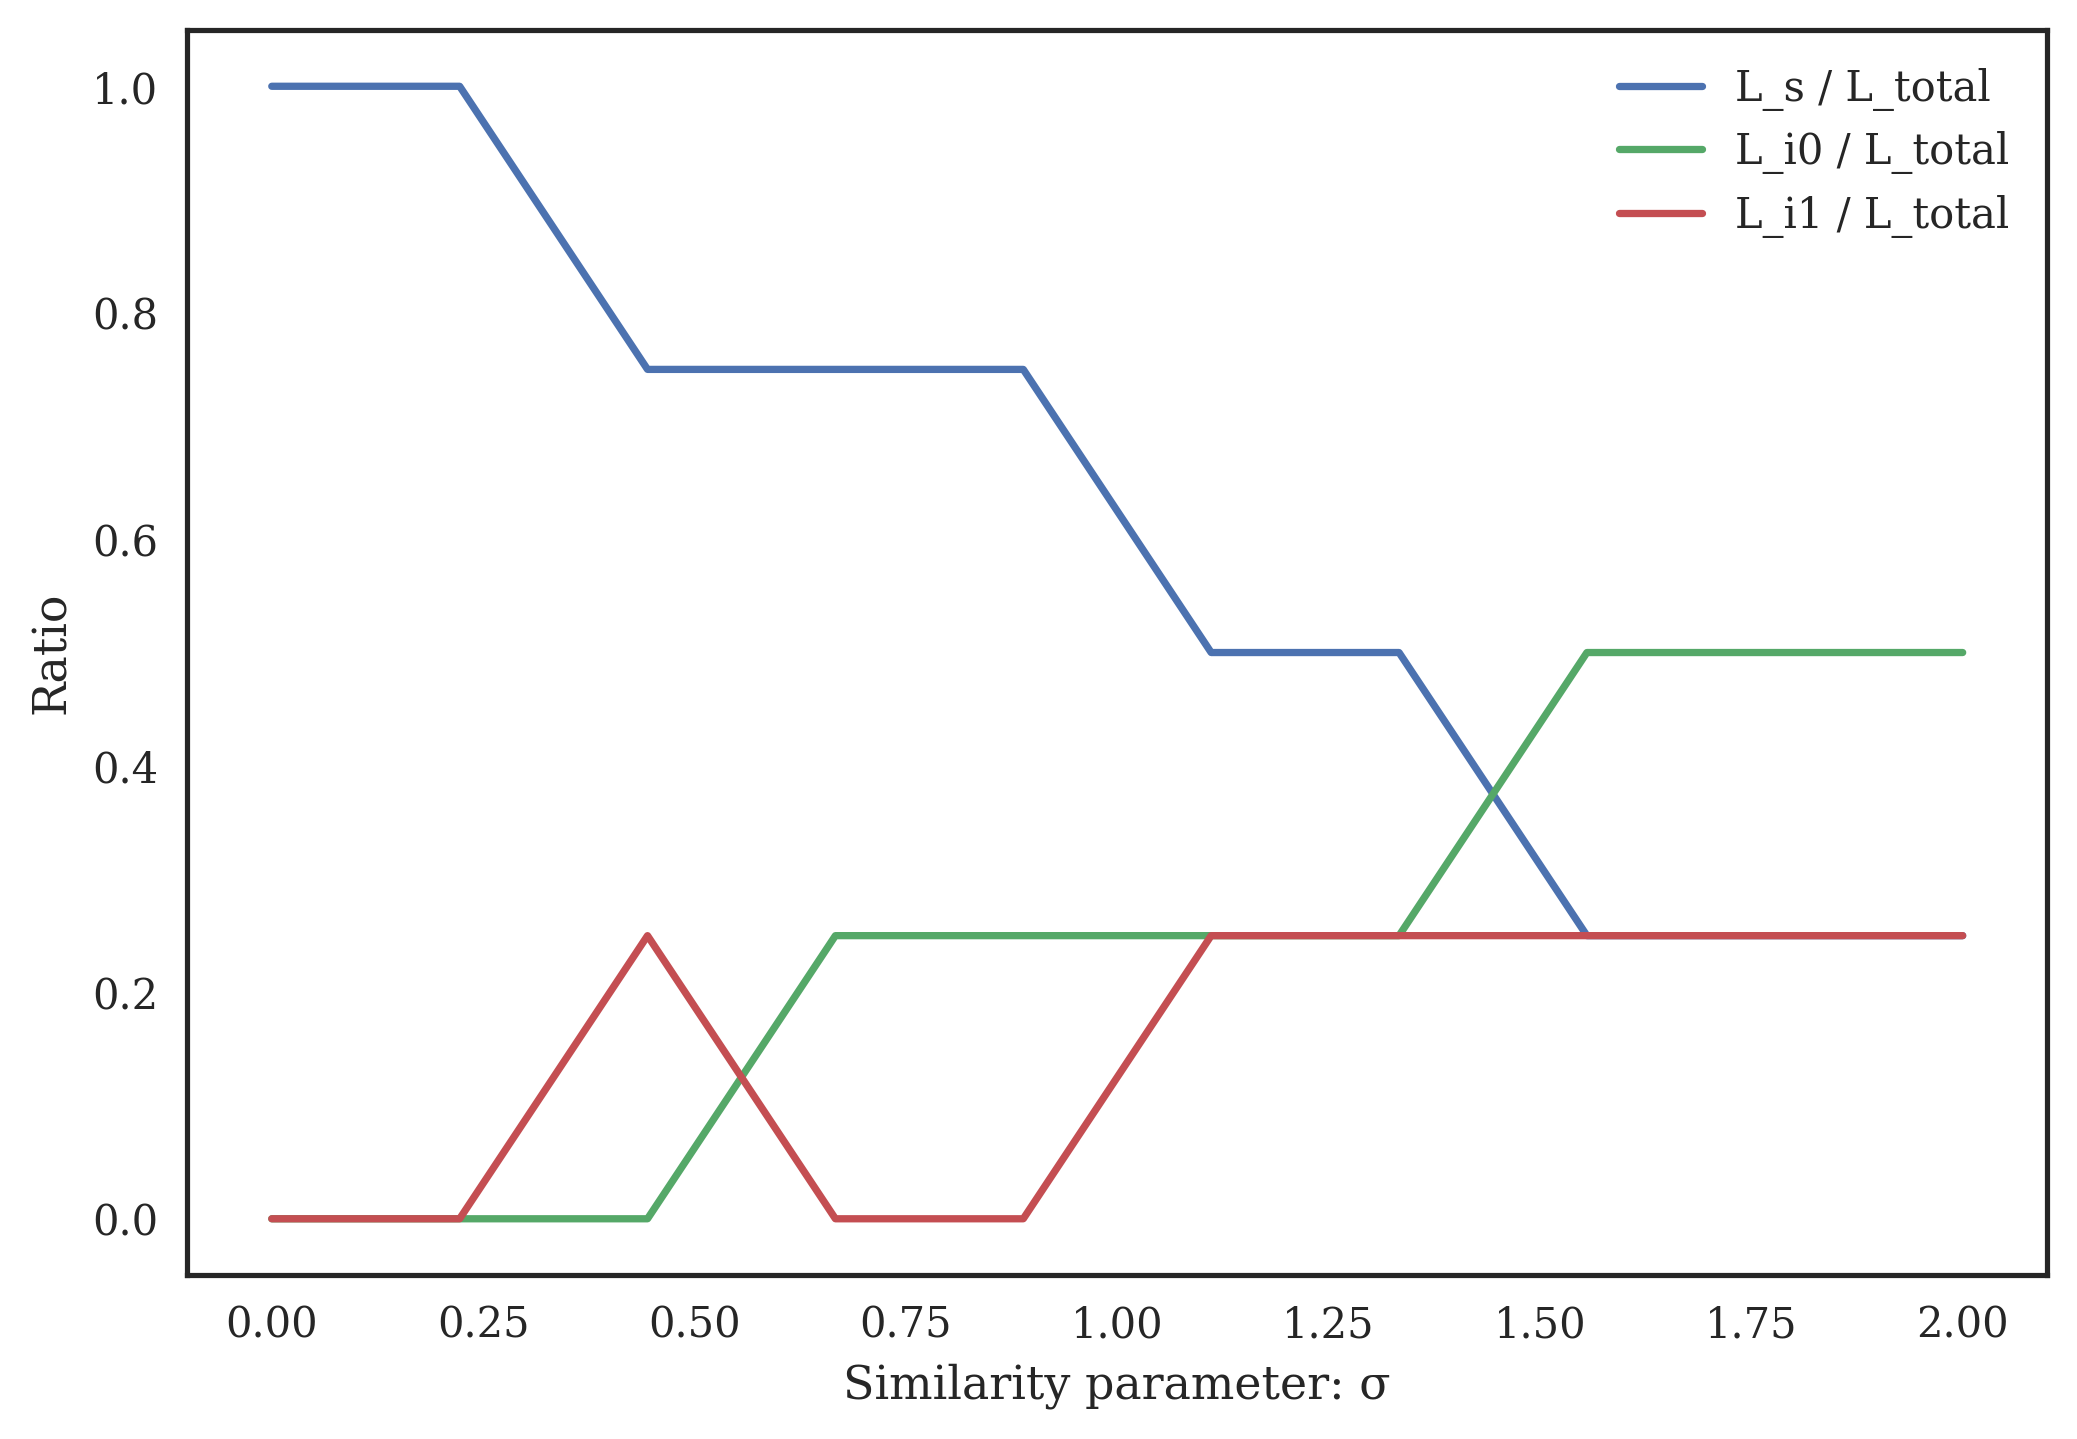
\includegraphics[width=.8\linewidth]{figures/chapter-5/syn-ratio-sigma.png}
		\caption{Learnt architecture (in terms of the ratios \textbf{R}) of the DCN-LA depending on the similarity parameter \textbf{S} of the input dataset. With decreasing similarity (higher sigma), the number of shared layers drops in favour of the outcome specific layers.}\label{fig:syn-sigma-ratios}
	\end{subfigure}
	\begin{subfigure}{\linewidth}
		\centering
		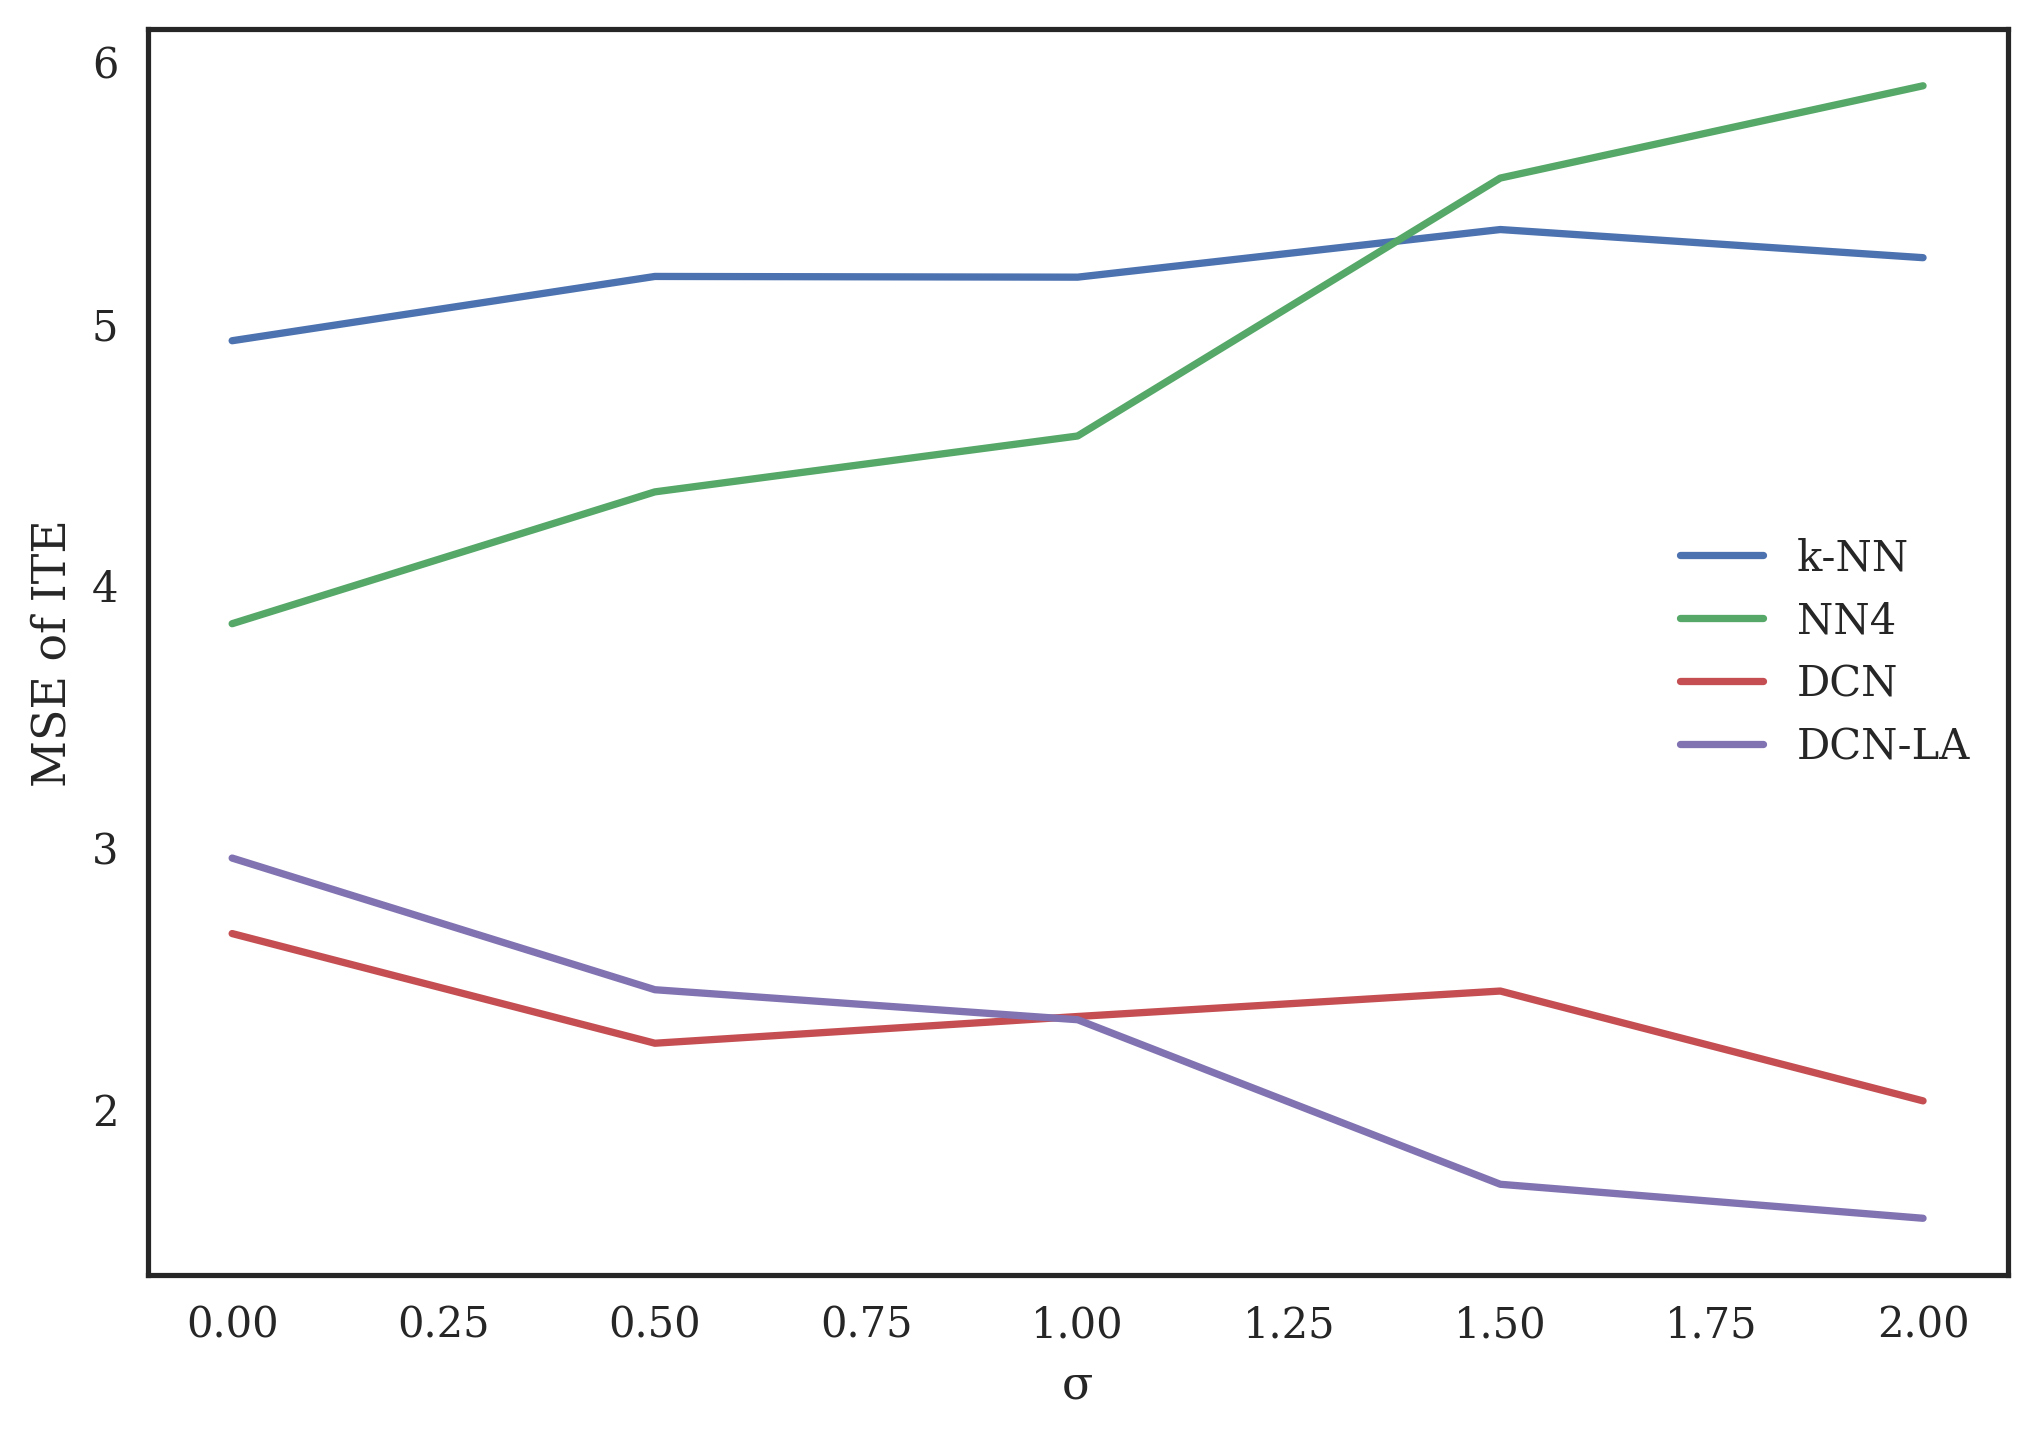
\includegraphics[width=.8\linewidth]{figures/chapter-5/syn-mse-sigma.png}
		\caption{Performances of DCN-LA, DCN, NN4, and k-NN for input datasets with different similarities. The DCN-LA is able to adapt well different response surfaces by utilising a higher number of outcome-specific layers. }\label{fig:syn-sigma-mse}
	\end{subfigure}  
 
\end{figure}  

\textbf{ii) Influence of the selection bias and response surface complexity:}
Figure \ref{fig:syn-beta} illustrates how the learnt architecture of the DCN-LA changes depending on the parameters $\mathbf{C}_0$ and $\mathbf{C}_1$ which measure the individual complexity of the respective outcome surface. As can be observed in the graph, the more complex the response surface of $Y^{(j)}$, the higher is the number of outcome-specific layers $L_{j,0}$ in the learnt model in relation to the shared layers and the outcome-specific layers of $Y^{(1-j)}$ leading to an asymmetric architecture. 

 \begin{figure}[h]
	\centering
	\caption[ The average and standard deviation of critical parameters ]
	{\small The average and standard deviation of critical parameters: Region R4} 
	\label{fig:syn-beta}
	\begin{subfigure}[b]{0.475\textwidth}
		\centering
		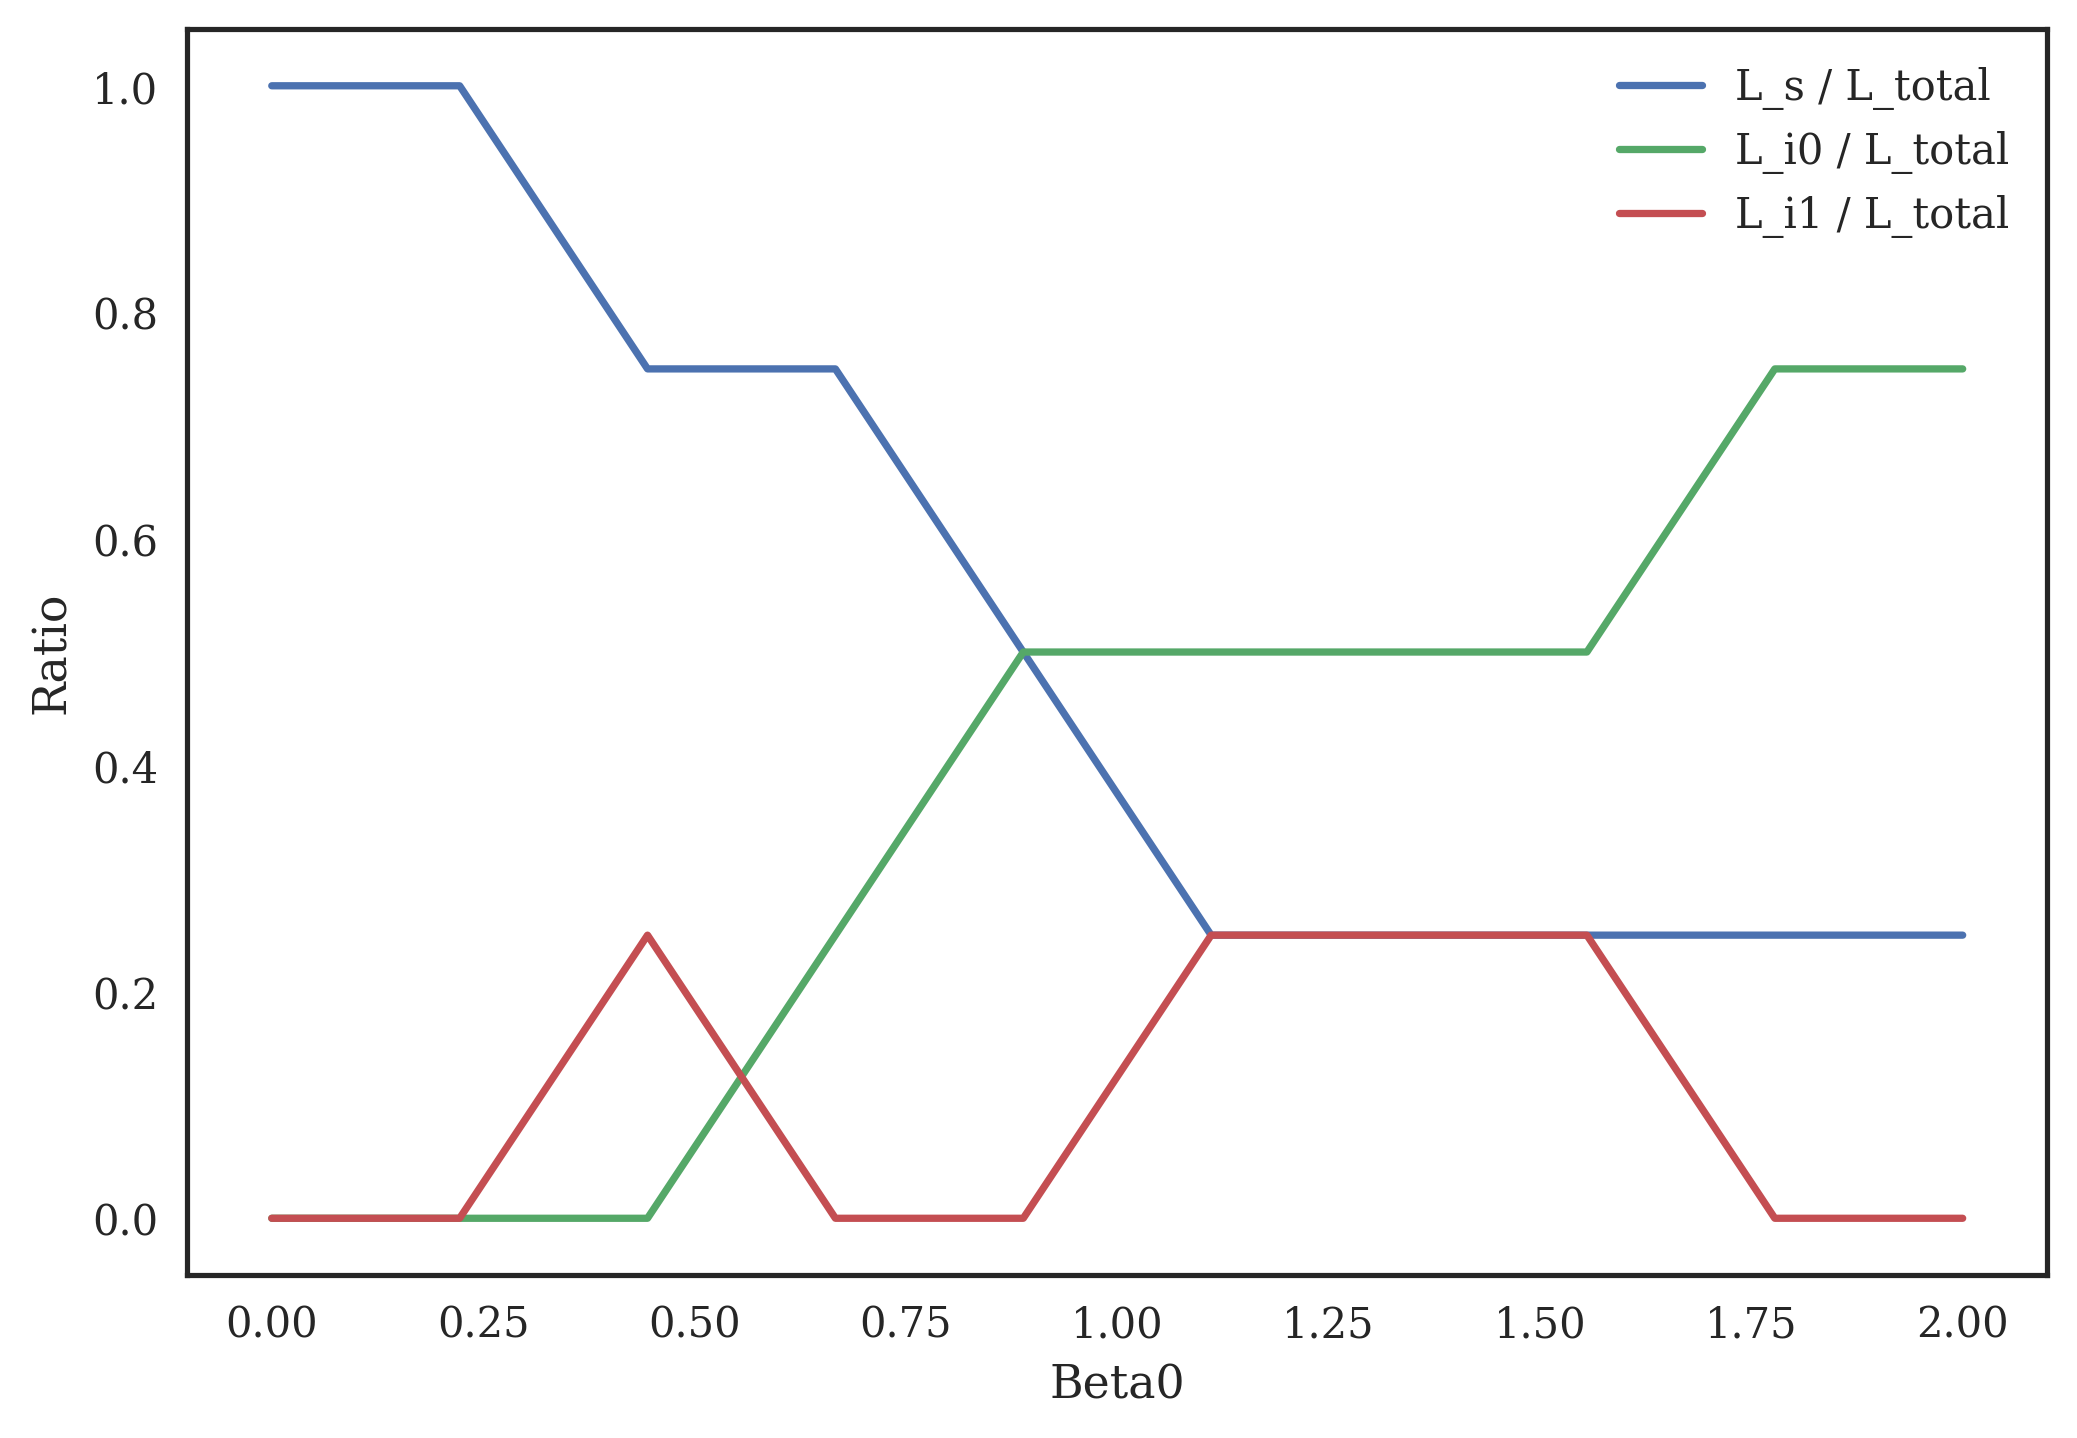
\includegraphics[width=\textwidth]{figures/chapter-5/syn-ratio-beta0.png}
		\caption[Network2]%
		{{Learnt architecture of DCN-LA depending on $\mathbf{C}_0$}}    
		\label{fig:mean and std of net14}
	\end{subfigure}
	\hfill
	\begin{subfigure}[b]{0.475\textwidth}  
		\centering 
		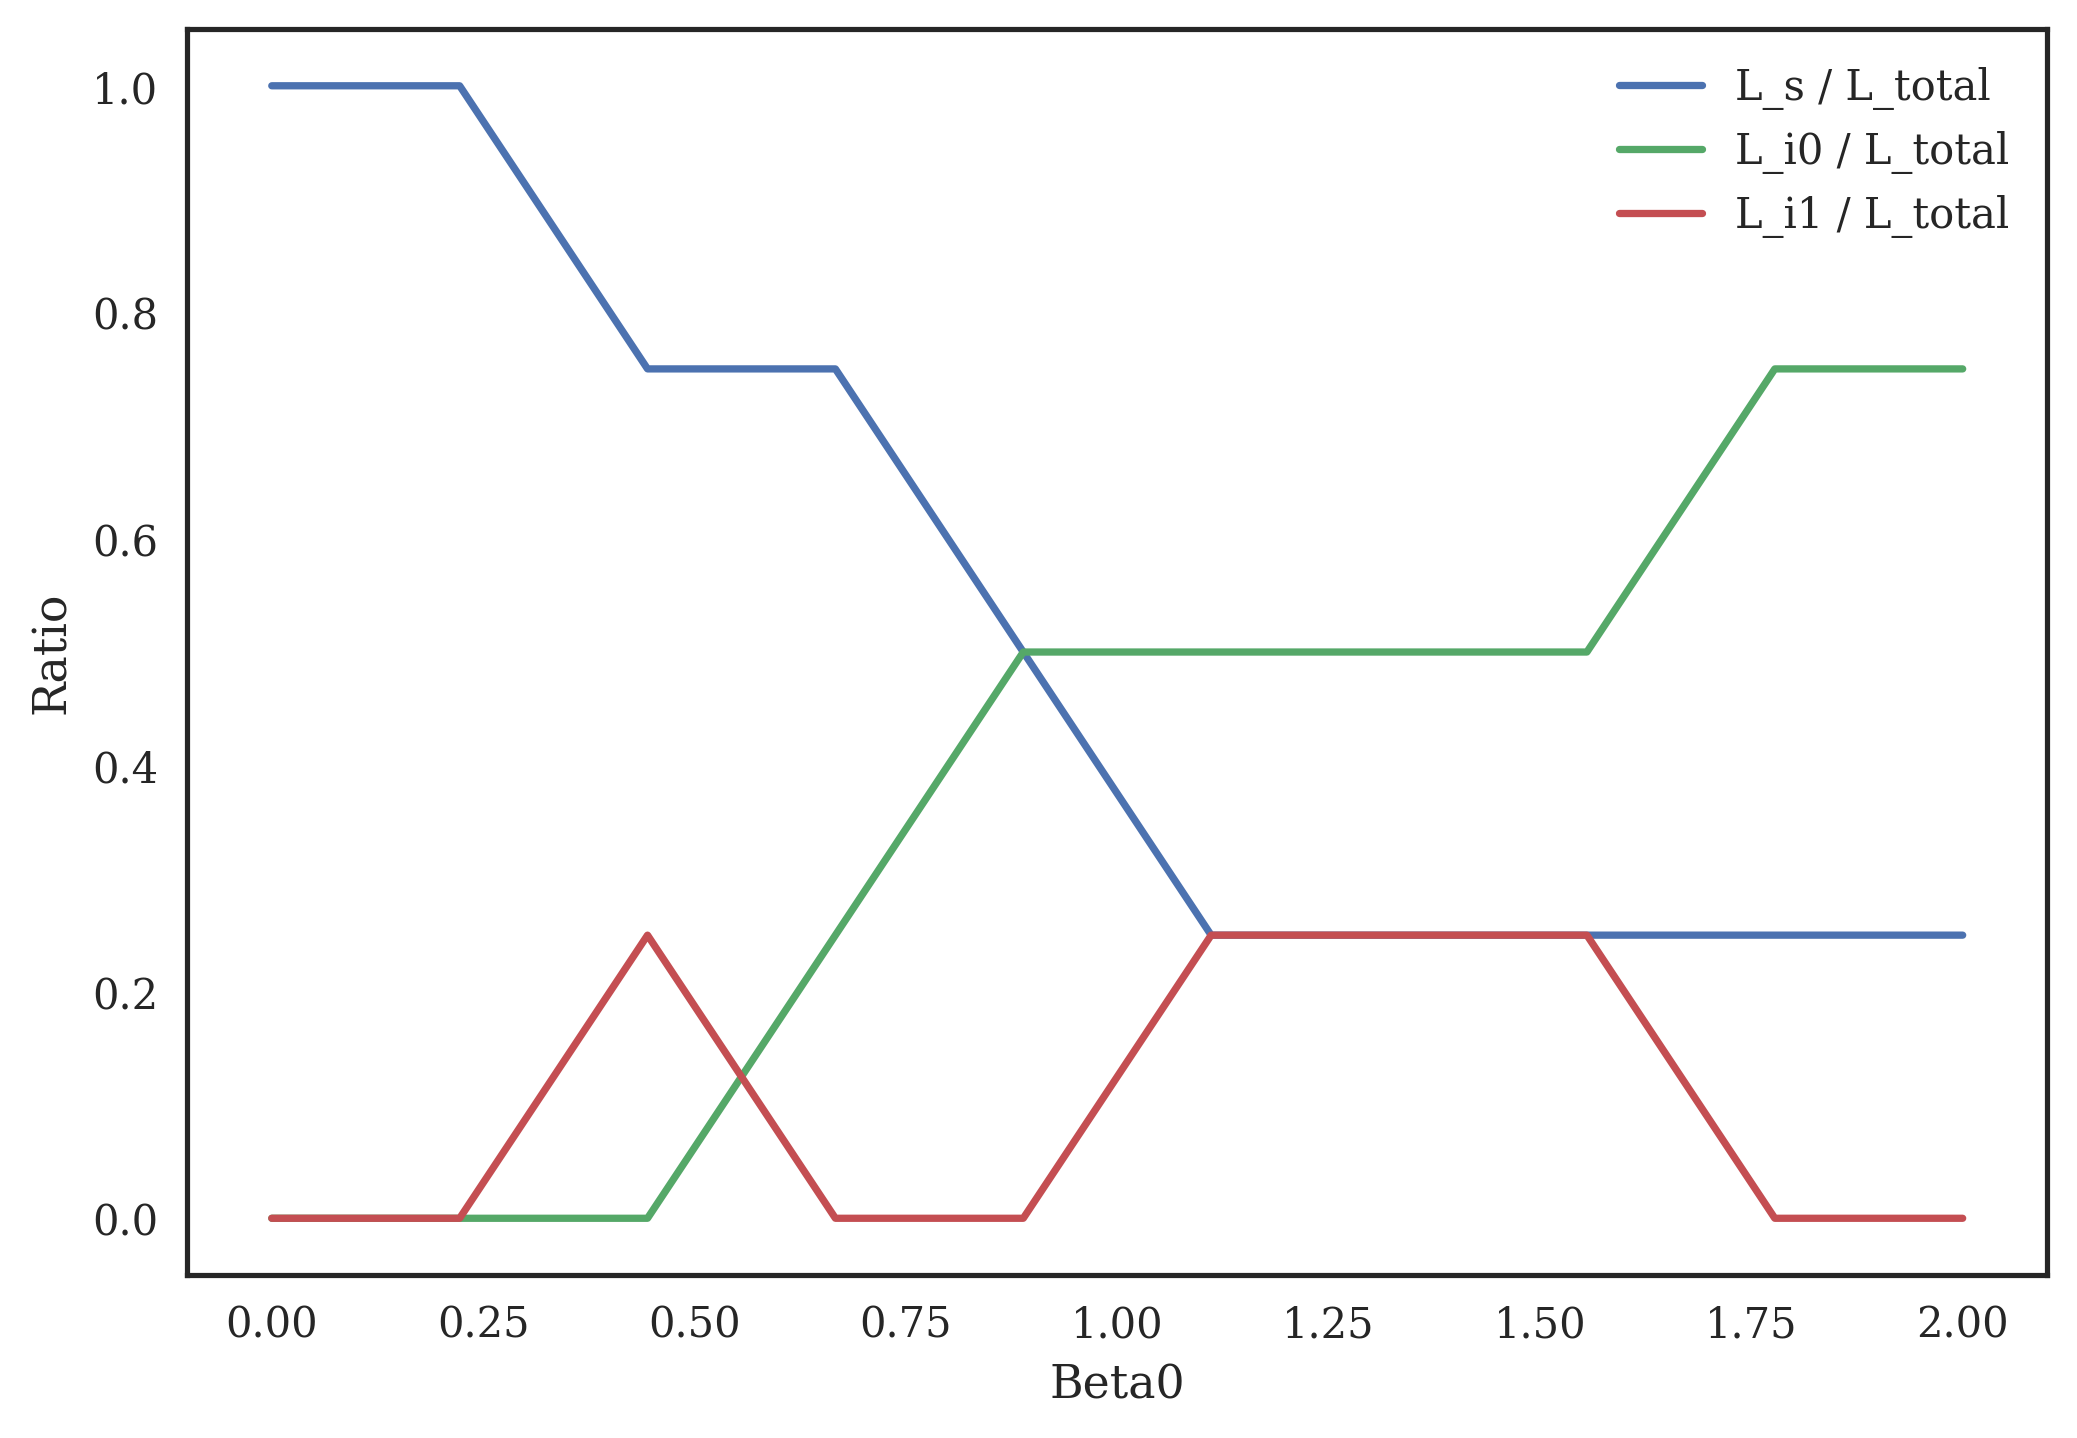
\includegraphics[width=\textwidth]{figures/chapter-5/syn-ratio-beta0.png}
		\caption[]%
		{Learnt architecture of DCN-LA depending on $\mathbf{C}_1$}    
		\label{fig:mean and std of net24}
	\end{subfigure}
	\vskip\baselineskip
	\begin{subfigure}[b]{0.475\textwidth}   
		\centering 
		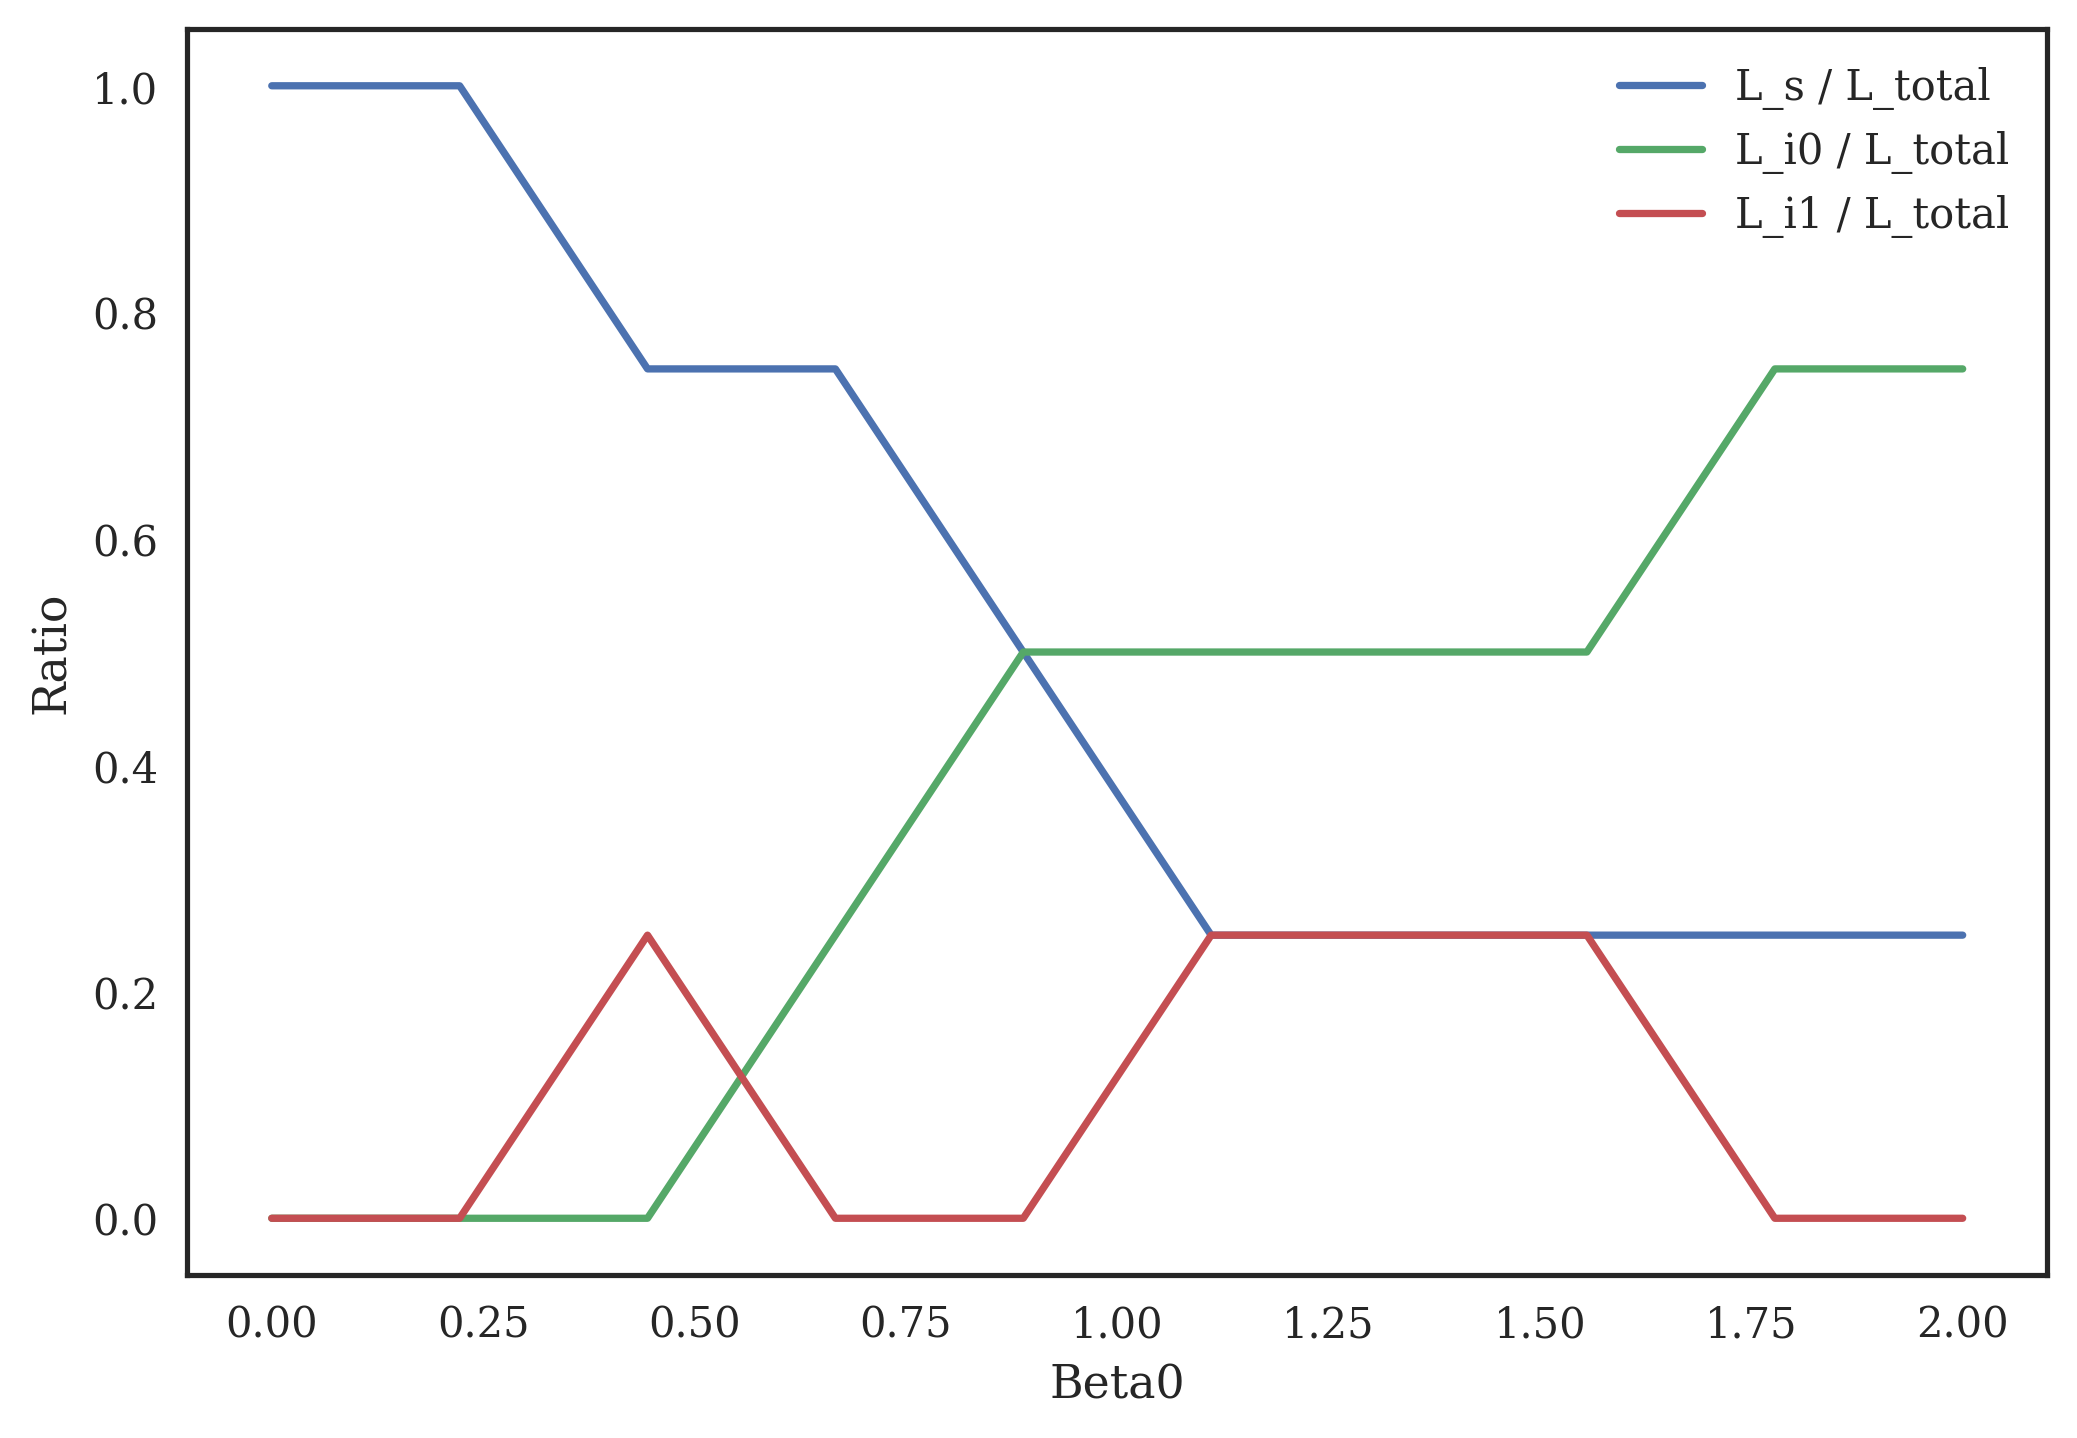
\includegraphics[width=\textwidth]{figures/chapter-5/syn-ratio-beta0.png}
		\caption[]%
		{Performance of DCN-LA depending on $\mathbf{C}_0$}    
		\label{fig:mean and std of net34}
	\end{subfigure}
	\quad
	\begin{subfigure}[b]{0.475\textwidth}   
		\centering 
		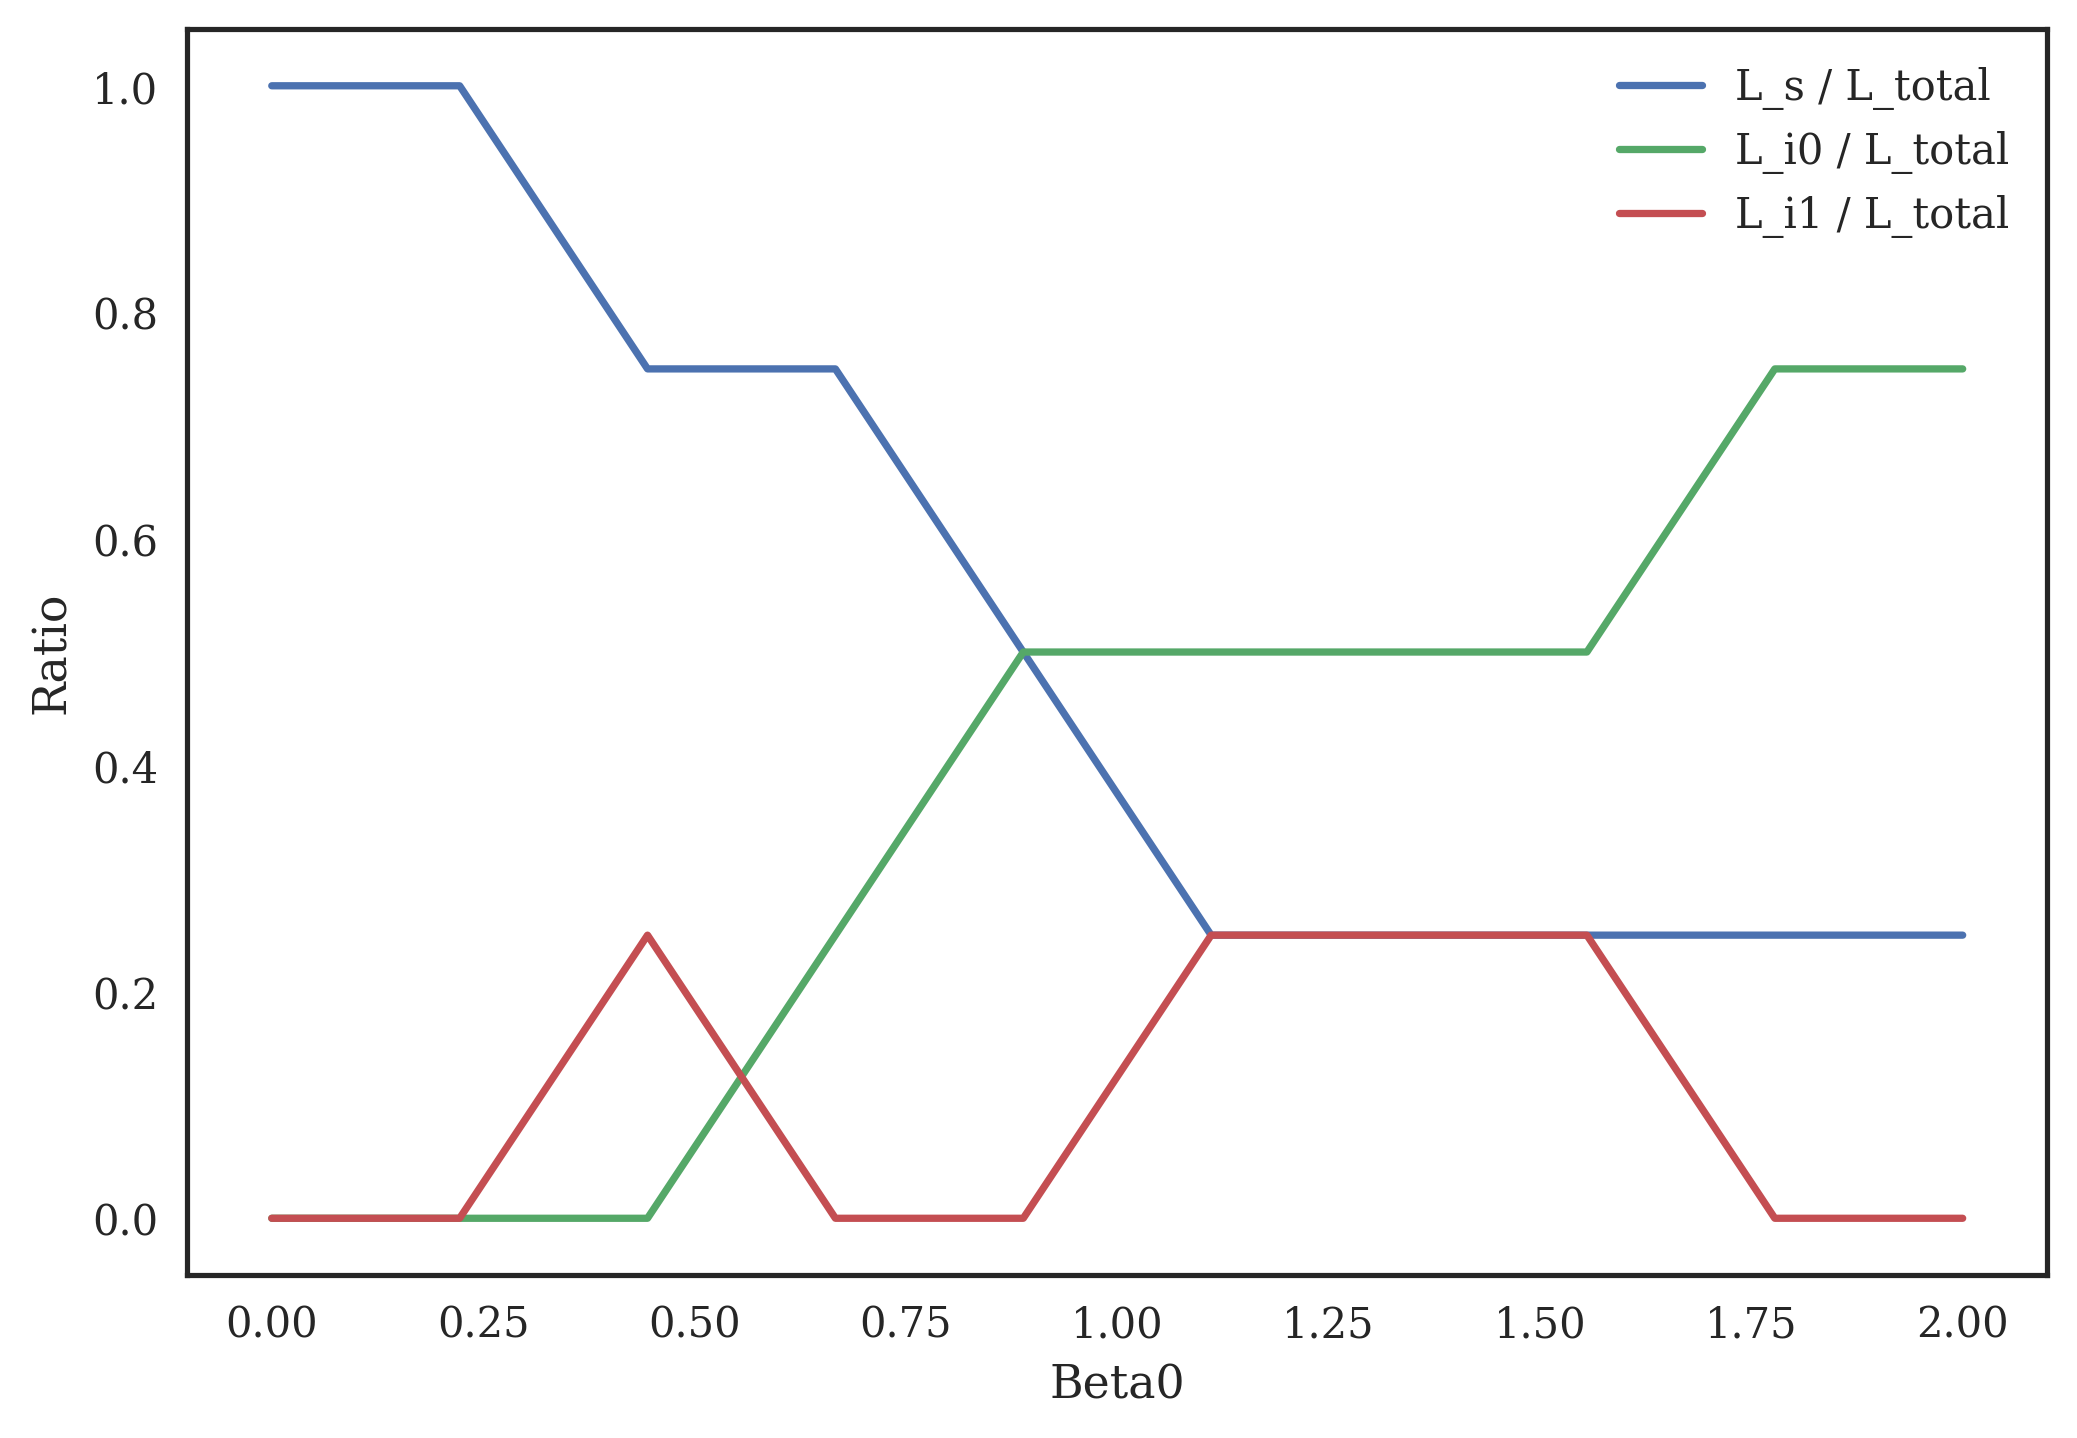
\includegraphics[width=\textwidth]{figures/chapter-5/syn-ratio-beta0.png}
		\caption[]%
		{Performance of DCN-LA depending on $\mathbf{C}_1$}    
		\label{fig:mean and std of net44}
	\end{subfigure}
	
\end{figure}

This observation corresponds well with our intuition that a more complex outcome requires a higher variance of the model reflected in a higher number of layers for the respective outcome. 


The differences between the learnt architectures for $\mathbf{C}_0$ and $\mathbf{C}_1$ can be explained in terms of the selection bias $\mathbf{B}$. The datasets used for the models on the right-hand side were generated with a selection bias of $\mathbf{B} = 0.75$ leading to a higher proportion of the subjects being treated than for the dataset shown on the left-hand side ($\mathbf{B} = 0.5$). As a consequence, the datasets with an strong selection bias are more imbalanced and have a higher number of subjects for the respective outcome, allowing the model to utilise a higher variance for the outcome with the larger population. 


\subsubsection{UNOS}
For the UNOS dataset we compare the performance of a DCN-LA, i.e. a DCN whose architecture was learnt according to our empirical model, to a standard DCN (see chapter \ref{ch:3-DCNs}), a feed-forward neural network with $4$ layers (NN-4), and a k-nearest-neighbour (k-NN) baseline approach.  

As we can see in table \ref{tab:dcn-la-results}, the DCN-LA achieves the lowest MSE outperforming the other methods. However, it has to be noted that the gain of the DCN-LA over the default DCN is only marginal. This might be due to the fact that the estimated characteristics, $\mathbf{B}, \mathbf{S}, \mathbf{C_0}, \mathbf{C_1}$ % TODO Should I provide concrete values? 
were relatively balanced reducing the potential of the method to learn a distinctive architecture. Nevertheless, the result implies that the approach of automatically deriving an appropriate architecture for a DCN can also be effectively applied to real-world dataset. 
%
%The BNN, representing  a strong benchmark as it effectively handles the selection bias by learning a balanced representation for the input features, represents the most competitive alternative. Lastly, the performance gains that our DCN-PD achieves over a the NN-4 model suggest that the multi-task learning framework is an effective conception of counterfactual inference that outperforms direct modelling approaches which consider the treatment assignment as a regular input feature.

\begin{table}[h]
	\centering
	\begin{tabular}{@{}cc@{}}
		\toprule
		\textbf{Algorithm} & \textbf{MSE}                \\ \midrule
		k-NN               &   $4.24 \pm 0.32$           \\
		NN-4                &  $3.19 \pm 0.16$           \\
		DCN                &   $2.63 \pm 0.08$           \\
		DCN-LA             &   $2.55 \pm 0.11$          \\\bottomrule
	\end{tabular}
	\caption{Performance of Deep Counterfactual Networks (DCN) and Deep Counterfactual Networks with Propensity-Dropout (DCN-DP) in comparison with baseline methods and existing competing approaches}\label{tab:dcn-la-results}
\end{table}

\subsection{Discussion}
The results above suggest that our proposed approach of automatically inferring an appropriate DCN architecture based on learnt characteristics of the dataset has the potential to significantly improve the performance of the model by reducing the MSE of the individualised treatment effect. 

As we have seen in the synthetic model, the DCN-LA performs particularly well when dealing with highly-imbalanced data (e.g. high propensity score, little shared complexity, and significantly different outcome surfaces). In these cases the DCN-LA is able to adapt an asymmetric architecture that significantly outperforms symmetric DCNs and other methods. 

However, the results on the UNOS dataset imply that our approach faces difficulties when dealing with real-world data that only expresses subtle imbalances that could be exploited. In these cases, a potential limitation may lie in the fact that the empirical model we use to infer appropriate ratios was pre-trained on \emph{synthetic} datasets that might display different properties and feature distributions than our real-world dataset. 

Nevertheless, even though the performance gain of the DCN-LA on the real-world dataset is marginal, the learnt architecture was derived without the need for computationally expensive hyper-parameter optimisation. So while our model might not always improve the solution quality, it has the potential to drastically reduce the computational costs of the training. 

Concluding, it can be said that our proposed approach of inferring architectures for DCNs by exploiting learnt characteristics of the dataset represents a promising approach that is able to compete with and -- depending on the properties of the dataset -- potentially outperform existing methods. 
